	%%%%%%%%%%%%%%%%%%%%%%%%%%%%%%%%%%%%%%%%%%%%%%%%%%%%%%%%%%%%%%%%
%
%  Template for homework of Introduction to Machine Learning.
%
%  Fill in your name, lecture number, lecture date and body
%  of homework as indicated below.
%
%%%%%%%%%%%%%%%%%%%%%%%%%%%%%%%%%%%%%%%%%%%%%%%%%%%%%%%%%%%%%%%%
\documentclass[11pt,letter,notitlepage]{article}
%Mise en page
\usepackage[left=2cm, right=2cm, lines=45, top=0.8in, bottom=0.7in]{geometry}
\usepackage{fancyhdr}
\usepackage{fancybox}
\usepackage{graphicx}
\usepackage{pdfpages}
\usepackage{enumitem}
\usepackage{algorithm}
\usepackage{algorithmic}
\renewcommand{\headrulewidth}{1.5pt}
\renewcommand{\footrulewidth}{1.5pt}
\newcommand\Loadedframemethod{TikZ}
\renewcommand{\thefootnote}{}

\usepackage[framemethod=\Loadedframemethod]{mdframed}
\usepackage{amssymb,amsmath,bm}
\usepackage{amsthm}
\usepackage{thmtools}
\usepackage{extarrows}
\usepackage{mathtools}
\usepackage{pifont}
\setlength{\topmargin}{0pt}
\setlength{\textheight}{9in}
\setlength{\headheight}{0pt}
\setlength{\oddsidemargin}{0.25in}
\setlength{\textwidth}{6in}
%%%%%%%%%%%%%%%%%%%%%%%%
%%%%%% Define math operator %%%%%
%%%%%%%%%%%%%%%%%%%%%%%%
\DeclareMathOperator*{\argmin}{\bf argmin}
\DeclareMathOperator*{\relint}{\bf relint\,}
\DeclareMathOperator*{\dom}{\bf dom\,}
\DeclareMathOperator*{\intp}{\bf int\,}
%%%%%%%%%%%%%%%%%%%%%%%
\setlength{\topmargin}{0pt}
\setlength{\textheight}{9in}
\setlength{\headheight}{0pt}
\setlength{\oddsidemargin}{0.25in}
\setlength{\textwidth}{6in}
\pagestyle{fancy}
%%%%%%%%%%%%%%%%%%%%%%%%
%% Define the Exercise environment %%
%%%%%%%%%%%%%%%%%%%%%%%%
\mdtheorem[
topline=false,
rightline=false,
leftline=false,
bottomline=false,
leftmargin=-10,
rightmargin=-10
]{exercise}{\textbf{Exercise}}
%%%%%%%%%%%%%%%%%%%%%%%
%% End of the Exercise environment %%
%%%%%%%%%%%%%%%%%%%%%%%
%%%%%%%%%%%%%%%%%%%%%%%%
%% Define the Problem environment %%
%%%%%%%%%%%%%%%%%%%%%%%%
\mdtheorem[
topline=false,
rightline=false,
leftline=false,
bottomline=false,
leftmargin=-10,
rightmargin=-10
]{problem}{\textbf{Problem}}
%%%%%%%%%%%%%%%%%%%%%%%
%% End of the Exercise environment %%
%%%%%%%%%%%%%%%%%%%%%%%
%%%%%%%%%%%%%%%%%%%%%%%
%% Define the Solution Environment %%
%%%%%%%%%%%%%%%%%%%%%%%
\declaretheoremstyle
[
spaceabove=0pt,
spacebelow=0pt,
headfont=\normalfont\bfseries,
notefont=\mdseries,
notebraces={(}{)},
headpunct={:\;},
headindent={},
postheadspace={ },
bodyfont=\normalfont,
qed=$\blacksquare$,
preheadhook={\begin{mdframed}[style=myframedstyle]},
postfoothook=\end{mdframed},
]{mystyle}
\declaretheorem[style=mystyle,title=Solution]{solution}
\mdfdefinestyle{myframedstyle}{%
	topline=false,
	rightline=false,
	leftline=false,
	bottomline=false,
	skipabove=-6ex,
	leftmargin=-10,
	rightmargin=-10,
	backgroundcolor=black!5}
%%%%%%%%%%%%%%%%%%%%%%%
%% End of the Solution environment %%
%%%%%%%%%%%%%%%%%%%%%%%

%% Homework info.
\newcommand{\posted}{\text{Oct. 15, 2024}}       			%%% FILL IN POST DATE HERE
\newcommand{\due}{\text{Oct. 24, 2024}} 			%%% FILL IN Due DATE HERE
\newcommand{\hwno}{\text{2}} 		           			%%% FILL IN LECTURE NUMBER HERE


%%%%%%%%%%%%%%%%%%%%
%% Put your information here %%
%%%%%%%%%%%%%%%%%%%
\newcommand{\name}{\text{San Zhang}}  	          			%%% FILL IN YOUR NAME HERE
\newcommand{\id}{\text{PBXXXXXXXX}}		       			%%% FILL IN YOUR ID HERE
%%%%%%%%%%%%%%%%%%%%
%% End of the student's info %%
%%%%%%%%%%%%%%%%%%%


\newcommand{\proj}[2]{\textbf{P}_{#2} (#1)}
\newcommand{\lspan}[1]{\textbf{span}  (#1)  }
\newcommand{\rank}[1]{ \textbf{rank}  (#1)  }
\newcommand{\RNum}[1]{\uppercase\expandafter{\romannumeral #1\relax}}
\DeclareMathOperator*{\cl}{\bf cl\,}
\DeclareMathOperator*{\bd}{\bf bd\,}
\DeclareMathOperator*{\conv}{\bf conv\,}
\DeclareMathOperator*{\epi}{\bf epi\,}


% \lhead{
% 	\textbf{\name}
% }
% \rhead{
% 	\textbf{\id}
% }
\chead{\textbf{Homework\hwno}}


\begin{document}
\vspace*{-4\baselineskip}
\thispagestyle{empty}


\begin{center}
{\bf\large Introduction to Machine Learning}\\
{Fall 2024}\\
University of Science and Technology of China
\end{center}

\noindent
Lecturer: Jie Wang  			 %%% FILL IN LECTURER HERE
\hfill
Homework \hwno             			
\\
Posted: \posted
\hfill
Due: \due
%\\
% Name: \name             			
% \hfill
% ID: \id						
% \hfill

\noindent
\rule{\textwidth}{2pt}

\medskip





%%%%%%%%%%%%%%%%%%%%%%%%%%%%%%%%%%%%%%%%%%%%%%%%%%%%%%%%%%%%%%%%
%% BODY OF HOMEWORK GOES HERE
%%%%%%%%%%%%%%%%%%%%%%%%%%%%%%%%%%%%%%%%%%%%%%%%%%%%%%%%%%%%%%%%

\textbf{Notice, }to get the full credits, please present your solutions step by step.
	
	\begin{exercise}[Projection ]
		Let $\mathbf{A}\in\mathbb{R}^{m\times n}$ and $\mathbf{x} \in \mathbb{R}^m$. Define
		\begin{align*}
			\proj{\mathbf{x}}{\mathbf{A}} = \argmin_{\mathbf{z}\in\mathbb{R}^m}\,\{\|\mathbf{x}-\mathbf{z}\|_2: \mathbf{z}\in\mathcal{C}(\mathbf{A})\}.
		\end{align*}
		We call $\proj{\mathbf{x}}{\mathbf{A}}$ the projection of the point $\mathbf{x}$ onto the column space of $\mathbf{A}$.
		\begin{enumerate}
			\item Please prove that $\mathbf{P}_{\mathbf{A}}(\mathbf{x})$ is unique for any $\mathbf{x} \in \mathbb{R}^m$.
			\item Let $\mathbf{v}_i \in \mathbb{R}^n$, $i=1,\ldots,d$ with $d\leq n$, which are linearly independent.
			\begin{enumerate}
				\item For any $\mathbf{w}\in \mathbb{R}^n$, please find $\proj{\mathbf{w}}{\mathbf{v}_1}$, which is the projection of $\mathbf{w}$ onto the subspace spanned by $\mathbf{v}_1$.
				\item Please show $\proj{\cdot}{\mathbf{v}_1}$ is a linear map, i.e.,
				\begin{align*}
					\proj{\alpha\mathbf{u}+\beta\mathbf{w}}{\mathbf{v}_1}=\alpha\proj{\mathbf{u}}{\mathbf{v}_1} + \beta \proj{\mathbf{w}}{\mathbf{v}_1},
				\end{align*}
				where $\alpha,\beta\in\mathbb{R}$ and $\mathbf{w}\in\mathbb{R}^n$.
				\item Please find the projection matrix corresponding to the linear map $\proj{\cdot}{\mathbf{v}_1}$, i.e., find the matrix $\mathbf{H}_1\in\mathbb{R}^{n\times n}$ such that
				\begin{align*}
					\proj{\mathbf{w}}{\mathbf{v}_1}=\mathbf{H}_1\mathbf{w}.
				\end{align*}
				\item Let $\mathbf{V}=(\mathbf{v}_1,\ldots,\mathbf{v}_d)$, and $\mathbf{v}_1,\ldots,\mathbf{v}_d$ are linearly independent.
                % added by haotonghuang
				\begin{enumerate}
					\item For any $\mathbf{w}\in \mathbb{R}^n$, please find $\proj{\mathbf{w}}{\mathbf{V}}$ and the corresponding projection matrix $\mathbf{H}$.
					\item Please find $\mathbf{H}$ if we further assume that $\mathbf{v}_i^{\top}\mathbf{v}_j=0$, $\forall\,i\neq j$.
				\end{enumerate}
			\end{enumerate}
			
			\item
			\begin{enumerate}
				\item Suppose that
				\begin{align*}
					\mathbf{A} = \left[
					\begin{matrix}
						1 & 0\\
						0 & 1
					\end{matrix}
					\right] .
				\end{align*}
				What are the coordinates of $\mathbf{P}_{\mathbf{A}}(\mathbf{x})$ with respect to the column vectors in $\mathbf{A}$ for any $\mathbf{x} \in \mathbb{R}^2$? Are the coordinates unique?
				\item Suppose that
				\begin{align*}
					\mathbf{A} = \left[
					\begin{matrix}
						1 & 2\\
						1 & 2
					\end{matrix}
					\right] .
				\end{align*}
				What are the coordinates of $\mathbf{P}_{\mathbf{A}}(\mathbf{x})$ with respect to the column vectors in $\mathbf{A}$ for any $\mathbf{x} \in \mathbb{R}^2$? Are the coordinates unique?
			\end{enumerate}
			
			\item (Optional) A matrix $\mathbf{P}$ is called a projection matrix if $\mathbf{P}\mathbf{x}$ is the projection of $\mathbf{x}$ onto $\mathcal{C}(\mathbf{P})$ for any $\mathbf{x}$.
			\begin{enumerate}
				\item Let $\lambda$ be the eigenvalue of $\mathbf{P}$. Show that $\lambda$ is either $1$ or $0$. (\emph{Hint: you may want to figure out what the eigenspaces corresponding to $\lambda=1$ and $\lambda=0$ are, respectively.})
				\item Show that $\mathbf{P}$ is a projection matrix if and only if $\mathbf{P}^2 = \mathbf{P}$ and $\mathbf{P}$ is symmetric.
			\end{enumerate}
			
			\item (Optional) Let $\mathbf{B} \in \mathbb{R}^{m\times s}$ and $\mathcal{C}(\mathbf{B}) $ be its column space. Suppose that $\mathcal{C}(\mathbf{B})$ is a proper subspace of $ \mathcal{C}(\mathbf{A})$.
			Is $\proj{\mathbf{x}}{\mathbf{B}}$ the same as $\proj{\proj{\mathbf{x}}{\mathbf{A}}}{\mathbf{B}}$? Please show your claim rigorously.
		\end{enumerate}
	\end{exercise}

\newpage
    \begin{exercise}[Projection to a Matrix Space]
        Let $\mathbb{R}^{n \times n}$ be the linear space of \(n \times n\) matrices. The inner product in this space is defined as \[ \langle A, B \rangle = \text{tr}(A^T B). \]
                \begin{enumerate}
                    \item Show that the set of diagonal matrices in $\mathbb{R}^{n \times n}$ forms a linear space. Besides, please find the the projection of any matrix onto the space of diagonal matrices.
                
                    \item Prove that the set of symmetric matrices, denoted $S^n$, in $\mathbb{R}^{n \times n}$ forms a linear space. Also, determine the dimension of this linear space.
    
                    \item Show that the inner product of any symmetric matrix and skew-symmetric matrix is zero. Moreover, prove that any matrix can be decomposed as the sum of a symmetric matrix and a skew-symmetric matrix.
    
                    \item Find the projection of any matrix onto the space of symmetric matrices.
                \end{enumerate}
    \end{exercise}

\newpage
    \begin{exercise}[Projection to a Function Space]

        \begin{enumerate}
            % \item Let $\mathbf{X}\in \mathbb{R}^{n\times d}$ with rank $d$ and $\mathbf{y}\in \mathbb{R}^n$. Consider the optimization problem
            % \begin{align*}
            %     \min_{\mathbf{w}\in \mathbb{R}^d}\|\mathbf{y}-\mathbf{X w}\|_2^2,
            % \end{align*}
            % \begin{enumerate}
            %     \item  We denote the column space of $\mathbf{X}$ by $\mathcal{C}(\mathbf{X})$. Please show that $\hat{\mathbf{y}}:=\mathbf{X}(\mathbf{X}^{\top}\mathbf{X})^{-1}\mathbf{X}^\top\mathbf{y}$ is the projection of $\mathbf{y}$ on $\mathcal{C}(\mathbf{X})$, i.e. $\langle\mathbf{y}-\hat{\mathbf{y}}, \mathbf{x}\rangle=0$ for any $\mathbf{x}\in\mathcal{C}(\mathbf{X})$.

            %     \item Please solve the above optimization problem by completing the square.

            %     \item Please show that $\min_{\mathbf{w}\in \mathbb{R}^d}\|\mathbf{y}-\mathbf{X w}\|_2\le \|\mathbf{y}\|_2$. Then find  the necessary and sufficient condition where the equality holds and give it a geometric interpretation.
            % \end{enumerate}

            \item Suppose $X$ and $Y$ are both random variables defined in the same sample space $\Omega$ with finite second-order moment, i.e. $\mathbb{E}[X^2], \mathbb{E}[Y^2]<\infty$.
            \begin{enumerate}
                \item Let $L^2(\Omega)=\{Z:\Omega\to\mathbb{R}\mid \mathbb{E}[Z^2]<\infty\}$ be the set of random variables with finite second-order moment. Please show that $L^2(\Omega)$ is a linear space, and $\langle X,Y \rangle:=\mathbb{E}[X Y]$ defines an inner product in $L^2(\Omega)$. Then find the projection of $Y$ on the subspace of $L^2(\Omega)$ consisting of all constant variables.
                \item Please find a real constant $\hat{c}$, such that
                \begin{align*}
                    \hat{c}=\argmin_{c\in \mathbb{R}}\mathbb{E}[(Y-c)^2].
                \end{align*}
                [Hint: you can solve it by completing the square.]

                \item Please find the necessary and sufficient condition where $\min_{c\in \mathbb{R}}\mathbb{E}[(Y-c)^2]=\mathbb{E}[Y^2]$. Then give it a geometric interpretation using inner product and projection.
            \end{enumerate}

            \item Suppose $X$ and $Y$ are both random variables defined in the same sample space $\Omega$ and all the expectations exist in this problem. Consider the problem
            \begin{align*}
                \min_{f:\mathbb{R}\to\mathbb{R}}\mathbb{E}[(f(X)-Y)^2].
            \end{align*}
            \begin{enumerate}
                \item Please solve the above problem by completing the square.
                \item We let $\mathcal{C}(X)$ denote the subspace $\{f(X)\mid f(\cdot):\mathbb{R}\to\mathbb{R}, \mathbb{E}[f(X)^2]<\infty \}$ of $L^2(\Omega)$. Please show that the solution of the above problem is the projection of $Y$ on $\mathcal{C}(X)$.
                \item Please show that question 1 is a special case of question 2. Please give a geometric interpretation of conditional expectation.  
            \end{enumerate}
        \end{enumerate}
    \end{exercise}	
	
\newpage
\begin{exercise}[Multicollinearity]
	Consider the linear regression problem formulated as below:
	$$\mathbf{y} = \mathbf{X} \mathbf{ w + e}, \mathbb{E}(\mathbf{e}) = \mathbf{0}, \operatorname{Cov}(\mathbf{e}) = \sigma^2 \mathbf{I_n}, $$where $\mathbf{y}=\left(y_{1}, \ldots, y_{n}\right)^{\top}$ and $\mathbf{X} \in \mathbb{R}^{n \times p}$. Suppose that $\mathbf{X}^{\top}\mathbf{X}$ is invertible, then $\hat{\mathbf{w}} = \left(\mathbf{X}^{\top} \mathbf{X}\right)^{-1} \mathbf{X}^{\top} \mathbf{y}$ is the least squares estimator of $\mathbf{w}$.
	\begin{enumerate}
		\item Recall that the covariance matrix of p-dimensional random vectors is defined as $$\operatorname{Cov}(\hat{\mathbf{w}}) = \mathbb{E}\mathbf{[(\hat{\mathbf{w}}-\mathbb{E}(\hat{\mathbf{w}}))(\hat{\mathbf{w}}-\mathbb{E}(\hat{\mathbf{w}}))^{\top}]}.$$
		Please show that
		\begin{enumerate}
			\item[(a)] $\mathbb{E}(\hat{\mathbf{w}}) = \mathbf{w}$;
			\item[(b)] $\operatorname{Cov}(\hat{\mathbf{w}}) = \sigma^2 \left(\mathbf{X}^{\top} \mathbf{X}\right)^{-1}$.
		\end{enumerate}
		\item We usually measure the quality of an estimator by mean squared error (MSE). The mean squared error (MSE) of estimator $\hat{\mathbf{w}}$ is defined as 	$$\text{MSE}(\hat{\mathbf{w}}) = \mathbb{E}[\left\|\hat{\mathbf{w}} - \mathbf{w}\right
		\|^2] .$$ Please derive that MSE can be decomposed into the variance of the estimator and the squared bias of the estimator, i.e.,
			$$\begin{aligned}
			\text{MSE}(\hat{\mathbf{w}}) &= \operatorname{trCov}(\hat{\mathbf{w}}) + \left\|\mathbb{E}\hat{\mathbf{w}}-\mathbf{w}\right\|^2\\
			&=\sum_{i=1}^{p} \operatorname{Var}(\hat{w_i}) + \sum_{i=1}^{p}  (\mathbb{E} \hat{w_i}-w_i)^2.
		\end{aligned}$$
		\item Please show that
		$$\text{MSE}(\hat{\mathbf{w}}) = \sigma^2 \sum_{i=1}^{p} \frac{1}{\lambda_i},$$
		
		where $\lambda_1,\lambda_2,\ldots,\lambda_{p}$ are the eigenvalues of $\mathbf{X}^{\top} \mathbf{X}$.
		\item What would happen if there exists an eigenvalue $\lambda_k \approx 0$?
	\end{enumerate}
\end{exercise}


	\newpage

	\begin{exercise}[Regularized least squares]
		Suppose that $\mathbf{X}\in \mathbb{R}^{n\times d}$.
		\begin{enumerate}
			\item Please show that $\mathbf{X}^{\top}\mathbf{X}$ is always positive semi-definite. Moreover, $\mathbf{X}^{\top}\mathbf{X}$ is positive definite if and only if $\mathbf{x}_1, \mathbf{x}_2, \dots, \mathbf{x}_d$ are linearly independent.
			\item Please show that $\mathbf{X}^{\top}\mathbf{X} + \lambda \mathbf{I}$ is always invertible, where $\lambda>0$ and $\mathbf{I}\in \mathbb{R}^{d\times d}$ is an identity matrix.
			\item (Optional) Consider the regularized least squares linear regression and denote
			$$
			\mathbf{w}^*(\lambda)=\argmin_\mathbf{w} L(\mathbf{w})+\lambda \Omega(\mathbf{w}),
			$$
			where $L(\mathbf{w})=\frac{1}{n}\|\mathbf{y}-\mathbf{Xw}\|_2^2$ and $\Omega(\mathbf{w})=\|\mathbf{w}\|_2^2$. For regular parameters $0<\lambda_1<\lambda_2$, please show that $L(\mathbf{w}^*(\lambda_1)) < L(\mathbf{w}^*(\lambda_2))$ and $\Omega (\mathbf{w}^*(\lambda_1)) > \Omega (\mathbf{w}^*(\lambda_2))$. Explain intuitively why this holds.
		\end{enumerate}
		
		
	\end{exercise}

\newpage
\begin{exercise}[High-Dimensional Linear Regression for Image Warping (Programming Exercise)]
Consider a data set $\mathcal{D} = \left\{\left(\mathbf{x}_i, \mathbf{y}_i\right)\right\}_{i=1}^{N}$ where $\mathbf{x}_i\in\mathbb{R}^n,\mathbf{y}_i\in\mathbb{R}^m,\; i=1,\;2,\;\dotsb N$, we want to find a map $\phi:\mathbb{R}^n\to \mathbb{R}^m$ such that
$\phi(\mathbf{x}_i) = \mathbf{y}_i,\; i=1,\;2,\;\dotsb N$.
Now given a set of basis functions $\phi_i: \mathbb{R}^n\to\mathbb{R}$
$$
\phi_i(\mathbf{x}) = \left(\Vert \mathbf{x} - \mathbf{x}_i \Vert _2^2 + r^2\right)^{\frac{\mu}{2}}
$$
where $\mu, r$ are costume constants. We can approximate function $\phi$ by a $\hat{\phi}(\mathbf{x})$:
$$
\hat{\phi}(\mathbf{x}) = \mathbf{A}\mathbf{x} + \mathbf{b} + \mathbf{W} \boldsymbol{\phi}(\mathbf{x})
$$
which is a linear combination of basis functions, where $\boldsymbol{\phi}(\mathbf{x}) := \left(\begin{matrix}\phi_1(\mathbf{x})& \phi_2(\mathbf{x}) &\dots &\phi_N(\mathbf{x})\end{matrix}\right)^T\in\mathbb{R}^N$, and parameters $\mathbf{W}\in\mathbb{R}^{m\times N}, \mathbf{A}\in\mathbb{R}^{m\times n}, \mathbf{b}\in\mathbb{R}^m$.
\begin{enumerate}
    \item Find $\mathbf{W}, \mathbf{A}, \mathbf{b}$ such that
\begin{align}
\min_{\mathbf{W}, \mathbf{A}, \mathbf{b}} l := \sum_{i = 1}^N\left\Vert \hat{\phi}(\mathbf{x}_i) - \mathbf{y}_i \right\Vert _2^2 + \lambda_1\Vert \mathbf{A} - \mathbf{I}\Vert_f^2 + \lambda_2 \Vert\mathbf{b} \Vert _2^2 + \lambda_3\Vert \mathbf{W}\Vert_f^2
\label{eq:EX6}
\end{align}
    where $\Vert \cdot\Vert_f$ is the Frobenius norm and $\lambda_1, \lambda_2, \lambda_3\in\mathbb{R}_+$.
    
    \textbf{Hint} (1) Take the partial derivatives with respect to $\mathbf{W}, \mathbf{A}, \mathbf{b}$, and set them to zero. (2) $\partial_\mathbf{X}\Vert \mathbf{X} - \mathbf{C}\Vert^2_f=2(\mathbf{X} - \mathbf{C})$.
    \item 
    
    Image warping is a technique used to smoothly distort or reshape an image based on specified transformation rules (shown in Figure \ref{fig:image-warping}). The user defines these rules by selecting points on the image, with each transformation mapping an initial position $\mathbf{x}_i$ to a target position $\mathbf{y}_i$. These point pairs form the training set $\mathcal{D} = \left\{\left(\mathbf{x}_i, \mathbf{y}_i\right)\right\}_{i=1}^{N}$, where $\mathbf{x}_i,\mathbf{y}_i \in \mathbb{R}^2$. A linear function $\hat{\phi}$ is then learned by minimizing the loss $l$ over the training set. This function is applied to every pixel $\hat{\mathbf{x_i}}$ in the test image, mapping it to an output coordinate $\hat{\mathbf{y_i}} = \hat{\phi}(\hat{\mathbf{x_i}})$. Finally, the pixel value at $\hat{\mathbf{y_i}}$ replaces that at $\hat{\mathbf{x_i}}$, generating the warped image.

    
    % First, the user needs to specify a set of control points {yi}Ni=1\{\mathbf{y}_i\}_{i=1}^N on the source image and drag them to the desired positions {xi}Ni\{\mathbf{x}_i\}_{i}^N, where xi,yi∈R2,i=1,2,⋯N\mathbf{x}_i,\mathbf{y}_i\in\mathbb{R}^2,\; i=1,\;2,\;\dotsb N.
    % Then, the software uses the linear regression method to find a map ˆϕ\hat{\phi} so that ˆϕ(xi)\hat{\phi}(\mathbf{x}_i) is as close as possible to yi\mathbf{y}_i. Finally, the algorithm iterates over every pixel coordinate x\mathbf{x} in the target image, computes the mapped value y=ˆϕ(x)\mathbf{y} = \hat{\phi}(\mathbf{x}), and sets the value of pixel x\mathbf{x} in the target image to the value of the pixel at coordinate y\mathbf{y} in the source image.

    Now let $r=0.5, \mu=1, \lambda
    _1 = \lambda_2 = \lambda_3 = 1e-2$. Please implement the image warping method in the provided framework. You can submit any image you like.
\end{enumerate}
\end{exercise}
\begin{figure}[htbp]
    \centering
        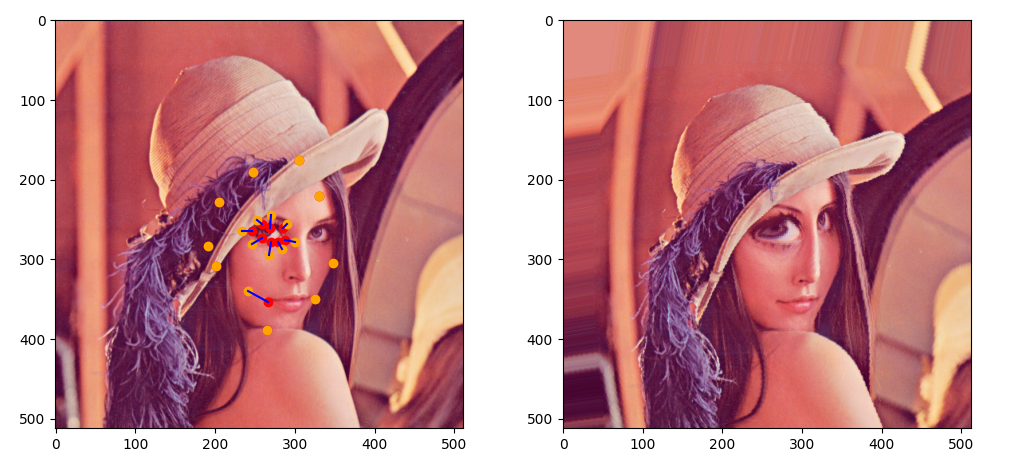
\includegraphics[width=0.6\textwidth]{./Figure/HW2-example.png}
        \caption{Image warping example}
        \label{fig:image-warping}
\end{figure}
    
\newpage
\begin{exercise}[Bias-Variance Trade-off (Programming Exercise) ]\label{BiasVariance}
    We provide you with $L=100$ data sets, each having $N=25$ points:
    $$
    \mathcal{D}^{(l)}=\{ (x_n,y_n^{(l)})\}_{n=1}^N,\quad l=1,2,\cdots ,L,
    $$
    where $x_n$ are uniformly taken from $[-1,1]$, and all points $(x_n, y_n^{(l)})$ are independently from the sinusoidal curve $h(x)=\sin (\pi x)$ with an additional disturbance.
    \begin{enumerate}
        \item For each data set $\mathcal{D}^{(l)}$, consider fitting a model with $24$ Gaussian basis functions
        \begin{align*}
            \phi_j(x)= e^{-(x-\mu_j)^2},\quad \mu_j = 0.2 \cdot (j-12.5),\quad j = 1,\cdots 24
        \end{align*}
        by minimizing the regularized error function
        \begin{align*}
            L^{(l)}(\mathbf{w}) = \frac{1}{2}\sum_{n=1}^N (y^{(l)}_n - \mathbf{w}^\top \bm{\phi}(x_n))^2 + \frac{\lambda}{2}\mathbf{w}^\top\mathbf{w},
        \end{align*}
        where $\mathbf{w}\in\mathbb{R}^{25}$ is the parameter, $\bm{\phi}(x)=(1, \phi_1(x),\cdots,\phi_{24}(x))^\top$ and $\lambda$ is the regular coefficient. What's the closed form of the parameter estimator $\hat{\mathbf{w}}^{(l)}$ for the data set $\mathcal{D}^{(l)}$?

        \item For $\log_{10}\lambda = -10, -5,-1,1$, plot the prediction functions $y^{(l)}(x)=f_{\mathcal{D}^{(l)}}(x)$ on $[-1,1]$ respectively. For clarity, show only the first $25$ fits in the figure for each $\lambda$.

        \item For $\log_{10}\lambda\in [-3,1]$, calculate the followings:
        \begin{align*}
            \bar{y}(x)& =\mathbb{E}_{\mathcal{D}}[f_{\mathcal{D}}(x)]=\frac{1}{L}\sum_{l=1}^L y^{(l)}(x) \\
            (\mbox{bias})^2& =\mathbb{E}_X[(\mathbb{E}_{\mathcal{D}}[f_{\mathcal{D}}(X)]-h(X))^2]=\frac{1}{N}\sum_{n=1}^N (\bar{y}(x_n)-h(x_n))^2\\
            \mbox{variance} &= \mathbb{E}_X[\mathbb{E}_{\mathcal{D}}[(f_{\mathcal{D}}(\mathbf{x})-\mathbb{E}_{\mathcal{D}}[f_{\mathcal{D}}(\mathbf{x})])^2]] = \frac{1}{N}\sum_{n=1}^N\frac{1}{L}\sum_{l=1}^L (y^{(l)}(x_n)-\bar{y}(x_n))^2
        \end{align*}
        Plot the three quantities, $(\mbox{bias})^2, \mbox{variance}$ and $(\mbox{bias})^2 + \mbox{variance}$ in one figure, as the functions of $\log_{10}\lambda$.
        (\textbf{Hint:} see \cite{Bishop2006} for an example.)
    \end{enumerate}

\end{exercise}



% \newpage
% \begin{exercise}[(Optional) Positive Semi-definite Matrices and the Polyhedron]
% Please show that Sn+\mathbb{S}_+^n is not a polyhedron.

% \end{exercise}

% \newpage
% \begin{exercise}[Convex Sets]
%     Let C⊂RnC \subset \mathbb{R}^n be a nonempty convex set. Please show the following statements.
%     \begin{enumerate}
%       \item Please find the interior and relative interior of the following convex sets (you don't need to prove them).
%       \begin{enumerate}
%           \item {x∈R3:x21+x22<1,x3=0}⊂R3\{\mathbf{x}\in\mathbb{R}^3: x_1^2+x_2^2<1,x_3=0\}\subset\mathbb{R}^3.
%           \item {A∈Sn++:Tr(A)=1}⊂Rn×n\{\mathbf{A}\in S_{++}^n: \text{Tr}(\mathbf{A})=1\}\subset \mathbb{R}^{n\times n}.
%           \item {A∈Sn++:Tr(A)=1}⊂Sn\{\mathbf{A}\in S_{++}^n: \text{Tr}(\mathbf{A})=1\}\subset S^ n.
%           \item (Optional) {A∈Sn++:Tr(A)≤1}⊂Rn×n\{\mathbf{A}\in S_{++}^n: \text{Tr}(\mathbf{A})\le1\}\subset \mathbb{R}^{n\times n}.
%           % \item \conv({x,x2,x3})⊂C[0,1]\conv (\{x, x^2, x^3\})\subset C[0,1] with L∞L^\infty norm, i.e., ‖\|f\|_\infty = \max_{x\in [0,1]}|f(x)| for any f\in C[0,1]f\in C[0,1].
%       \end{enumerate}
%       \item  Some operations that preserve convexity.
%       \begin{enumerate}
%         \item
%         Both \clC\cl C  and \intpC\intp C  are convex.
%         \item
%         The set \relintC\relint{C} is convex.
%         \item
%         The intersection ⋂i∈ICi\bigcap_{i \in I}C_i of any collection {Ci:i∈I}\{ C_i:i\in \mathcal{I} \} of convex sets is convex.

%         \item
%         The set {y∈Rm:y=Ax+a,x∈C}\{ \mathbf{y}\in\mathbb{R}^m:\mathbf{y}=\mathbf{Ax}+\mathbf{a},\mathbf{x}\in C \} is convex, where A∈Rm×n\mathbf{A} \in \mathbb{R}^{m \times n} and a∈Rm\mathbf{a} \in \mathbb{R}^m.
%         \item
%         The set {y∈Rm:x=By+b,x∈C}\{ \mathbf{y}\in\mathbb{R}^m:\mathbf{x}=\mathbf{By}+\mathbf{b},\mathbf{x}\in C \} is convex, where B∈Rn×m\mathbf{B} \in \mathbb{R}^{n \times m} and b∈Rn\mathbf{b} \in \mathbb{R}^n.
%     \end{enumerate}

%     \end{enumerate}

% \end{exercise}
% \begin{solution}

% \end{solution}

% \footnotetext{You will attain \textbf{one extra point} of bonus in your \textbf{final rating} if you work out this problem.}
%%%%%%%%%%%%%%%%%%%%%%%%%%%%%%%%%%%%%%%%%%%%%%%%%%%%%%%%%%%%%%%%
	
	\newpage
	\begin{thebibliography}{1}
	\bibitem{Bishop2006}
	C.~M. Bishop.
	\newblock {\em Pattern Recognition and Machine Learning}.
	\newblock Springer, 2006.
	\end{thebibliography}
	

\end{document}
